\section{The Large Hadron Collider}

Located in the Lemanic basin, straddling the border between Switzerland and France, the Large Hadron Collider is the largest machine built by humans.
The LHC provides the unique laboratory conditions in which detectors like ATLAS investigate the fundamental nature of our Universe.
The construction, maintenance, and operation of the LHC continues to be an enormous task carried out by thousands of dedicated scientists and engineers. Without their ongoing efforts, the achievements of ATLAS and the other LHC experiments would be impossible.

The LHC is impressive not just in absolute terms, but also in comparison to previous accelerators.
The three other large superconducting accelerators, the Tevatron\footnote{Decommissioned in 2011.}, HERA, and RHIC, all operate with fields of approximately 5~T. The LHC exceeds this with fields of 8~T.
The machine is also enormous. It has a circumference of 26.7~km. It takes 15 days to cool down a sector.
The LHC, designed to reach collision energies of 14 TeV, is also the first hadron accelerator with enough synchrotron radiation to effect the design of the cooling and vacuum systems \cite{lyndon}.

The LHC is composed of a number of subsystems, each of which is complex and essential in its own right.
In particular, the following systems will be described here:
\begin{itemize}
    \item The magnet system, which is responsible for bending the beam around the path of the machine.
    \item The vacuum system, which evacuates the beampipe.
    \item The radio-frequency system, which accelerate the beams. 
    \item The power system that powers the machine.
    \item The beam instrumentation, collimation, and control systems that monitors and adjusts the beam.
    \item The beam injection and extraction systems.
\end{itemize}
The LHC is a machine under continuous development. The only place to study improvements for the LHC is at the LHC.
As a result, the history of the LHC development is also the history of the experimental environment of the ATLAS detector.
This story begins with the tunnel and infrastructure that house the LHC.

\subsection{Civil Engineering}

\begin{figure}[h!]
\captionsetup[subfigure]{position=b}
\centering
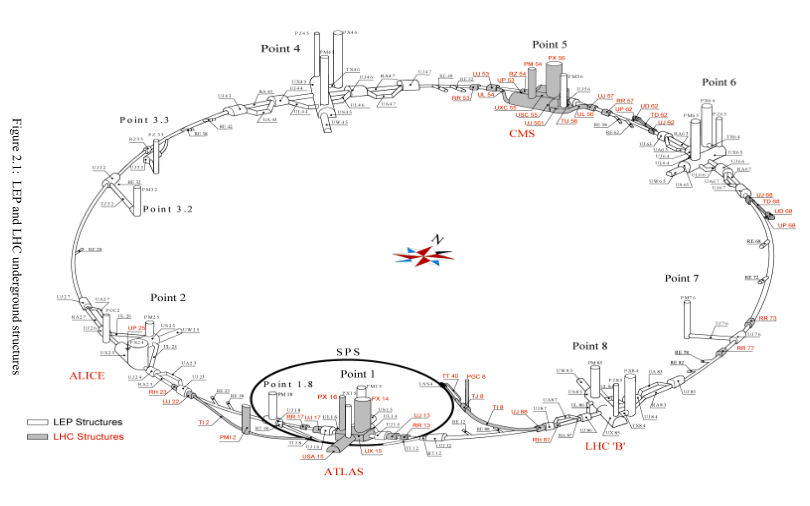
\includegraphics[width=0.9\textwidth]{figures/experiment/lhcLepLayout.png}
\caption{The LHC infrastructure layout. Figure from the LHC Design Report \cite{lhcDesignV2}.}
\label{figure:lhcLayout}
\end{figure}


The first step in building a collider is civil infrastructure.
This takes the form of building that house services for the accelerator, and a space for the machine itself.
For economical reasons, much of the infrastructure for the LHC is reused from the earlier LEP project.

The largest piece of infrastructure is the tunnel built to house LEP.
The Tevatron is buried less than 10~m deep in the flat expanse of the Illinois prairie. This shallow tunnel could be constructed with a cut-and-fill approach.
RHIC is primarily build at surface level in a tunnel that was later covered with dirt.
Neither of these approaches were suitable in the context of the geology of the region.
The land near CERN consists of a layer of moraine (loose unconsolidated rock) resting atop a layer of molasse (soft sedimentary rock).
LEP was buried in the sedimentary layer for stability, but this is too deep for excavation.
Instead, beginning in 1985, the tunnel was dug using tunnel bores and explosives.
In the Cenozoic molasse of the Lemanic basin, tunnel bores were the fastest option.
The tunnel bores were unsuitable for the fractured Mesozoic limestone beneath the Jura mountain, and explosives were used instead.
The resulting tunnel's internal diameter is 3.8~m, and it is buried at a depth of 45-170~m.
The tunnel slopes downward at 1.42 degrees in the direction of Lake Leman, in order to remain within the molasse layer.

The tunnel has eight curved arcs, separated by eight straight sections with length 528~m. \cite{lyndon}
Four straight sections house the ATLAS, CMS, ALICE, and LHCb experiments. These are 
The other four straight sections house the RF system, collimation controls, beam abort, and other utilities.
The eight straight sections arrayed as shown in Figure \ref{figure:lhcLayout} numbered p$i$ with $i\in\{1,...,8\}$.
The primary uses of each point is:
\begin{itemize}
    \item \textbf{p1} hosts the ATLAS experiment
    \item \textbf{p2} injection, and the ALICE experiment
    \item \textbf{p3} hosts momentum collimation
    \item \textbf{p4} hosts RF systems
    \item \textbf{p6} hosts beam abort, and beam dump
    \item \textbf{p5} hosts the CMS and TOTEM experiments
    \item \textbf{p7} hosts betatron collimation
    \item \textbf{p8} injection, and the LHCb experiment
\end{itemize}
The eight curved sections host magnets with the purpose of bending the beam around the path of the machine.
The accelerator itself is built along the outer edge of the tunnel. In several locations, concentric outer tunnels house services for the accelerator.

After below ground infrastructure, the next largest infrastructure for the LHC is surface buildings.
Every LEP building has been reused for the LHC.

New infrastructure was built to accommodate the LHC.
First, a major expansion of the tunnels was undertaken to carry the beam from the SPS to the injection points of the LHC. Two new tunnels with internal diameter of 3.75~m and length of 2.5~km were dug to connect points p2 and p8 to the SPS.
While ALICE and LHCb reuse existing LEP era caverns, new caverns were built to house ATLAS and CMS.
In the case of the cavern for CMS, the water logged moraine above the cavern had to be frozen with liquid nitrogen before excavation could be completed.
To avoid further flooding\footnote{LEP flooded twice, at one time filling with 20~cm of sediment. A plan to waterproof the tunnel with a steel tube called ``the submarine'' was rejected.} existing draining tunnels were enlarged, and new tunnels were added.

In total, the new infrastructure lasted five years, with the exception of the CMS cavern.
Work at p1 for the three ATLAS caverns began in April of 1998.
Four new shafts, two over the experimental cavern and one over each service cavern were dug.
Eight new surface building were constructed to hold offices and experimental equipment.

\subsection{Accelerator Design}
The heart of the LHC is the accelerator.
The purpose of this system is to accelerate beams to their collision energy, and then maintain their energy to compensate for losses over time.
Beams are accelerated only in a short section of p4.
The circular design of the LHC means that beams repeatedly pass through the same acceleration section.
During the design operation, synchrotron radiation energy loss is 3.7 kW/beam: not much acceleration is lost in a revolution.
The acceleration system needs only to make up for a small amount of lost energy per turn.

The principle of acceleration is based on radio-frequency (RF) cavities.
Independent RF systems control the acceleration of each beam.
% Each cavity provides 32kW to increase the beam energy.
Cavities are made of copper, sputtered\footnote{A vapor deposition technique, in magneton sputtering a material (niobium) is vaporized by particle bombardment and bound to a substrate (copper) resulting in a 1-2 mircon thin - and cheap - coating.} with niobium.
This is advantageous over solid niobium for its thermal conductivity, but also superconductive to enhance the RF performance.\cite{lyndon}
The operation of the superconducting cavities requires temperatures of 4.5~k, so cavities are enclosed in cryomodules with their own helium tanks. \cite{boussard}
The resonant properties of the cavities can adjusted during operation by mechanically distorting their shape.

Each cavity operates with a voltage of 2~MV (5.3 MV/m), and is powered by a 500~kW klystron.
The klystrons are coupled to the cavities by a waveguide of adjustable length.
Adjusting the length of the waveguide in turn adjusts the \emph{quality factor}\footnote{Peak energy lost per cycle, which can be used to adjust the peak voltage in the cavity.} of the cavity.
The cavity is kept at a 3~kV bias to reduce the rate of electron avalanches (multipactor effect).
During normal operation, the klystrons drive the cavities at 400~MHz and supply 200~kW.

\begin{figure}[h!]
\captionsetup[subfigure]{position=b}
\centering
    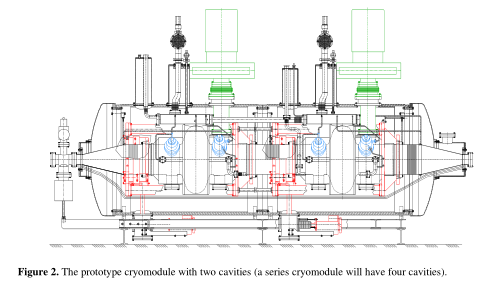
\includegraphics[width=1\textwidth]{figures/experiment/rfproto.png}
\caption{Schematic of a prototype RF cryostat, containing only two cavities. Figure from the The LHC Superconducting RF System \cite{boussard}.}
\label{fig:cavities}
\end{figure}

There are eight single cell cavities per beam.
Four cavities are grouped to share a single cryostat, which maintains their superconducting temperature.
The resulting total voltage gradient is 16~MV per beam.
A simplified schematic is shown in Figure \ref{fig:cavities}.
The driving frequency is supplied through the couplings on top of the cryostat.
The cryostats are too large to sit next to each other in the tunnel, so they are staggered.

\subsection{Magnet Design}
If the accelerator is the heart of the LHC, the magnets compose its body.
Magnets serve multiple purposes in handling the beam.
\begin{itemize}
    \item Dipole magnets bend the beam around the curved sections.  There are 1232 main dipoles.
    \item Quadrupole magnets focus and defocus the beam. Each quadrupole simultaneously focuses in one direction and defocuses in an orthogonal direction. There are 392 arc quadrupoles throughout the LHC.
    \item Sextupole for correcting chromaticity introduced by quadrupoles. There are 2464 in total.
    \item Other magnets such as octupole and decapole correctors fill in the remaining 7000 superconducting magnets.
\end{itemize}
Together these magnets steer the beam into the LHC and maintain the beam's orbit during collisions.
At the end of the beam's lifetime, kicker magnets steer the beam safely into the beamdump.

\begin{figure}[h!]
\captionsetup[subfigure]{position=b}
\centering
\subcaptionbox{One element group\label{fig:dipoleFlux2}}{
    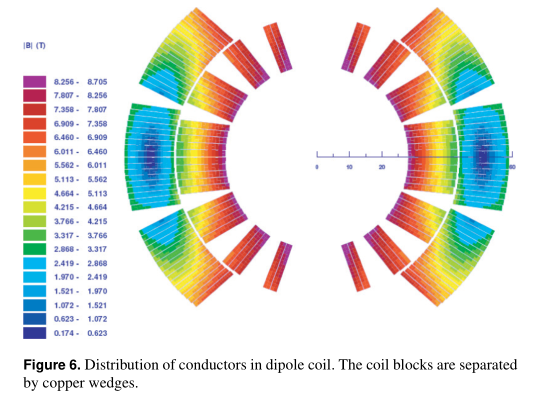
\includegraphics[width=0.4\textwidth]{figures/experiment/coils.png}
}
\subcaptionbox{One element group\label{fig:dipoleFlux1}}{
    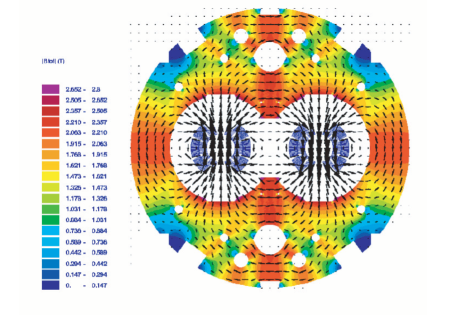
\includegraphics[width=0.4\textwidth]{figures/experiment/field.png}
}
\caption{Illustration of the magnetic flux in the dipole magnets. Figure from the The Large Hadron Collider \cite{lyndon}}
\label{fig:dipoleFlux}
\end{figure}

% Dipole system
The job of bending the beam around the LHC is performed by the dipole magnets.
Because the counter circulating beams are both positively charged, magnetic fields of opposite directions are needed to steer them.
In the dipole magnets, two sets of superconducting coils are wound from niobium-titanium (Nb-Ti) alloy wires\footnote{Although niobium-tin (Nb$_3$Si) has many desirable advantages over Nb-Ti, it is brittle and requires many hours of heat treatment at 970~k. On the other hand, Nb-Ti has low heat capacity at 1.8~k, so it is susceptible to rapid heating and quenching}.
The coils are arranged in inner and outer layers as shown in Figure \ref{fig:dipoleFlux2}.
This configuration produces a homogeneous, purely dipole field.
The coils for each beam are positioned side-by-side, such that the field of one can augment that of the other.
These coils share a common yoke made from low carbon steel with high magnetic permeability, chosen to conduct the magnetic flux between the coils.
This is illustrated by the black arrows in Figure \ref{fig:dipoleFlux1}.
The coil and yoke assembly is held in place by collar plates of austenitic (low permeability) steel.
The resulting magnetic field has an incredible strength 8.3~T.
Each of the main dipole magnets has a length of 14.2~m (15~m including connections between the magnets).

% Cryosystem
In order to operate at superconducting temperatures, the magnets are housed elaborate cryosystems.
These are challenging systems: during the LHC's Run 1, the cryosystem was responsible for 25-30\% of fault time.\cite{lhcRun1}
It is the task of the cryosystem to maintain the magnet at 1.9~k using superfluid helium. A total of 100 tons is used throughout the LHC.
Helium is used because its low viscosity allows it to permeate the coil insulation and contact directly with the superconducting wire.
Since superfluid helium has a specific heat roughly 2000 times that of the Nb-Ti, this has the important benefit of increasing the specific heat of the system.
Helium is also effective at quickly transporting heat away from the wired.
The magnets are submerged in a bath of 1~bar liquid helium. A pipe with is pumped with low pressure 15~mbar liquid helium to pull heat away from the bath.
This is done to keep prevent vapor bubbles from developing in the bath, which could lead to the coil heating and subsequent quenching.
In the event of a quench, a capacitor bank is fired into series with the coil to make it resistive. The current is diverted through a diode while the power is ramped down.

Magnets are grouped together into ``periods'' with identical magnetic properties.
Each period is 106.9~m long and consists of six main dipoles, and two 6.6~m ``short straight sections'' (SSS).
Each SSS contains quadrupole magnets that re-focus the beam after being steered by the dipoles.
In addition, each SSS also contains sextupoles that control chromaticity, and small dipoles for orbit corrections.
Some SSS also contain octupoles, and trip/skew quadrupoles for fine tuning the beam characteristics.
Perturbations in the trajectory of the beam are introduced by the magnets and are called \emph{dispersion}.
After completing one of the eight arcs, the magnet of the dispersion suppressor system cancel horizontal dispersion introduced by during the bending.

\subsection{Beam Structure and Design}
The achievement of building the LHC pales in comparison to the achievement of producing and maintaining its beams.
The LHC was designed to collide two counter-rotating beams, at precise locations, with the enormous instantaneous luminosity of $10^{34}cm^{-2}s^{-1}$.
The energy of each beam exceeds that of a large truck traveling at highway speeds.
This is more than one hundred fold the stored beam energy of any previous machine. \cite{lyndon}
The beam is an object of enormous energy, and surpassing delicacy.
There are numerous technical considerations that must be addressed in order for the beam to useful for the experiments.
The beams at the LHC are characterized by a number of parameters that describe its stability and utility.
These parameters are described in this section.

The first parameter to consider is the \emph{emittance}, $\epsilon$, defined in Equation \ref{eqn:emittance}.
It is a measure of the distribution of the particles in a beam in position-momentum phasespace.
The emittance is given as
\begin{equation}\begin{split}\label{eqn:emittance}
\epsilon = \frac{6\pi}{B}(w^2-D^2(\frac{dp}{p})^2),
\end{split}\end{equation} 
where $w$ is the RMS beam width, $D$ is the dispersion, $B\approx(w/\epsilon)$ is the beta function, and $\frac{dp}{p}$ is the relative momentum spread.
The emittance is often divided into longitudinal and transverse components.
If the emittance is too small, then intra-beam interactions destabilize the beam. 
During injection, the beam has a longitudinal emittance of 0.6-1 eV, and this is increased to 2.5 eV during acceleration for stability.
Conversely, if the transverse emittance is too large then colliding beams pass through each other without interacting.
\cite{boussard}\cite{lyndon}\cite{pdgAccelSection}

\begin{figure}[h!]
\captionsetup[subfigure]{position=b}
\centering
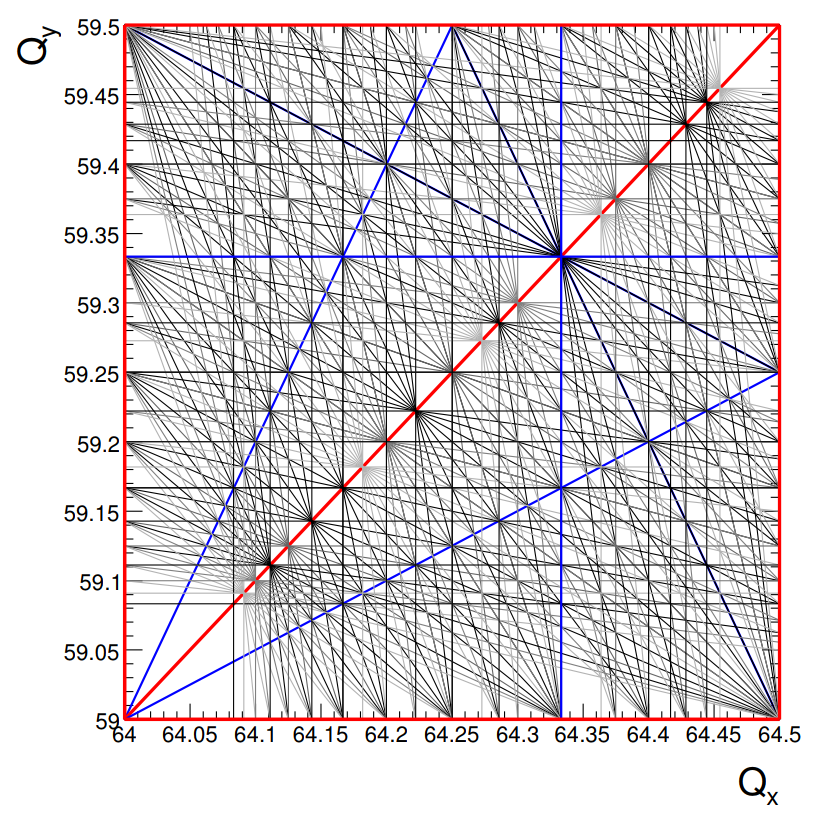
\includegraphics[width=0.4\textwidth]{figures/experiment/tune.png}
\caption{Tune diagram for the LHC. The horizontal and vertical tunes are displayed. First order resonances shown in red, second order resonances shown in blue, and higher order resonances shown in black. Figure from \emph{Tune and Chromaticity Diagnostics} \cite{steinhagen}}
\label{fig:tune}
\end{figure}

Related to the transverse emittance are \emph{betatron oscillations}: harmonic motion in the transverse plane as the beam makes an orbit.\cite{pdgAccelSection}
This is a problematic source of intra-beam scattering of protons through coulomb forces.
The frequency of betatron oscillations is higher than that of the orbit.
The number of vertical or horizontal betatron oscillations made during one orbit is called the vertical or horizontal \emph{tune} respectively.
The horizontal and vertical tunes must be carefully picked using a tune diagram, such as shown in Figure \ref{fig:tune}.
Resonances are illustrated as lines, and the tunes must be selected together to avoid disruptive resonances.

Related to the longitudinal emittance are \emph{synchrotron oscillations}: longitudinal oscillation along the direction of the beam.
This takes place at a much lower frequency than that of betatron oscillations: at the LHC it is less than one oscillation per orbit.
As with betatron oscillations, the synchrotron oscillation frequency must be carefully controlled to limit intra-beam scattering, and maintain beam stability.\cite{pdgAccelSection}

\emph{Chromaticity} describes the dependence of the tune on a change of momentum.
In optics, light rays of different wavelengths are focused differently by a glass focusing lens.
There is a persistent analogy between optics and beam dynamics (often called beam optics). Like light, beams are bent and focused by magnets. 
Particles with large momentum experience weaker focusing strength from focusing quadrupoles, a process called \emph{chromatic aberration}.
Chromaticity quantifies this momentum dependence.
To put it explicitly, chromaticity $Q'$ is the tune change $\Delta Q$ caused by a momentum change $\Delta p/p$. \cite{fuchsberger}
\begin{equation}
    \Delta Q = Q'\frac{\Delta p}{p},
\end{equation}
where
\begin{equation}
\begin{split}
    \frac{\Delta p}{p} = \frac{\frac{\Delta f}{f}}{\eta}; \quad\text{and}\quad \eta = \frac{1}{\gamma_r}-\alpha_c. \\
\end{split}
\end{equation}
Here, $\Delta f$ is change in RF frequency, and $f$ is the nominal frequency \footnote{400,788,860 Hz at the LHC.} 
$\gamma_r$ is relativistic gamma function, and $\alpha_c$ is momentum compaction factor equal to $3.225\times10^{-4}$ at the LHC.
Chromaticity is unitless as it defines a change in the tune.
At the LHC, sextupoles are used to control the beam's correct chromatic aberration after passing through focusing quadrupoles and dispersion suppression. \cite{frascati} \cite{bruno}
The chromaticity is visualized on a tune diagram, such as Figure \ref{fig:tune}, as the area occupied by the beam.
Reducing the beam's chromaticity makes it easier to find a stable setting for the tune.
% From Jorg
Beams with a chromaticity that is too small, however, suffer from instability related interaction with the beampipe.
The momentum spread of a beam with high chromaticity makes it more efficient to absorb reflected EM fields without perturbing the beam.
An important task is to find a balance for the chromaticity in order to maximize the useful life of the beam.

% Bunches
Because the RF cavities produce alternating field gradients, the beam is naturally organised into occupied \emph{bunches} and empty space.
The time interval between these, the bunch spacing, is a multiple of the RF frequency.
At the LHC the nominal bunch spacing is 24.96~ns, or ten times the RF frequency. The corresponding bunch length is 7.5~cm. \cite{boussard}
Bunches are collected into trains, patterns of occupied and empty bunches.
Several trains comprise the beam.
Several bunches are always left unoccupied, called the abort gap. The length of the gap corresponds to the ramp time of the extraction kicker magnet.
The bunch design choice depends on the function of the beam. Some patterns are useful for, example, cleaning the beampipe of electron clouds, while others are useful for optimizing physics collisions.

% Lumi
From a physics perspective, the most important beam characteristic is the instantaneous luminosity of collisions.
This is defined as $L\equiv N/\sigma_{pp}$, where $N$ is the collisions per second and $\sigma_{pp}$ is the poorly defined proton-proton collision cross-section\footnote{This is poorly defined because in some sense protons always scatter off each other, so the definition depends on what constitutes a collision. Traditionally, values of $\sigma_{pp}\sim10^{14}\text{fb}$ are used.} \cite{lyndon}
More precisely in the context of the LHC, the luminosity is defined in Equation \ref{eqn:lumi}.\cite{lyndon}
\begin{equation}\label{eqn:lumi}
    L=\frac{N_b^2nf_r\gamma}{4\pi\epsilon_n\beta^*}
\end{equation}
Here, $N_b$ is number of particles per bunch, and $n$ is the number of bunches per beam.
$f_r$ is is revolution frequency, which is 11.245 kHz for the LHC.
The other terms are the previously mentioned relativistic $\gamma$, the transverse emittance $\epsilon_n$, and the beta function at the collision point $\beta^*$.
The two beams must be steered into each other at a crossing angle $\theta_c$.
This results in a luminosity reduction factor,
\begin{equation}\label{eqn:lumiReduce}
    F=1/\sqrt{1+\frac{\theta_c\sigma_Z}{2\sigma^*}}
\end{equation}
where $\sigma_z$ is the RMS bunch length, and $\sigma^*$ is the transverse RMS beam size at the interaction point.
In fact, $\sigma^*$ is specifically minimized by focusing the beam before the collisions, and defocusing it afterwards.

The challenge during the operation of the LHC is to keep the beam in a stable orbit for many hours.
A number of issues can effect the stability of the beam during this time. \cite{lyndon}
\begin{itemize}
    \item \textbf{Beam-beam interaction:} the force from electromagnetic field from one beam on another. Beam-beam interaction can be reduced by increasing the crossing angle $\theta_c$, but this reduces the luminosity as shown in Equation \ref{eqn:lumiReduce}.
    \item \textbf{Intra-beam interaction:} coulomb scattering during betatron and synchrotron oscillations. While protons migrate within a bunch, they can knock other protons into different betatron orbits. 
    \item \textbf{Coherent instabilities:} the beam interacts with its environment, generating EM fields, that in turn act on the beam. The induced fields are mitigated by smoothing the beampipe as much as possible, to the extent where interconnects are covered with smooth segments. The impact of coherent instabilities on the beam is decreased by increasing chromaticity.
    \item \textbf{Electron clouds:} the accumulation of electrons in beam pipe. The major sources are ionization of gas in pipe, and excitation from synchrotron radiation knocking electrons off beam pipe. The issue is that the beam can collide with these free electrons, and accelerate them. The energetic electrons then collide with the beampipe and produce an electron shower, leading to exponential growth of the cloud. This is especially problem if the mean drift time for electrons is resonant with beam bunch spacing. Electron clouds are a large source of heat for the cryogenic equipment. Electron clouds are combatted by improving the vacuum, and picking bunch structures that do not resonate with with the clouds. As a further measure, warm chambers (including in the detectors) are coated with TiZrV, a ``getter'' material that passively pump vacuum and absorbs electron clouds.
\end{itemize}


\subsection{Beam Abort}

\begin{figure}[h!]
\captionsetup[subfigure]{position=b}
\centering
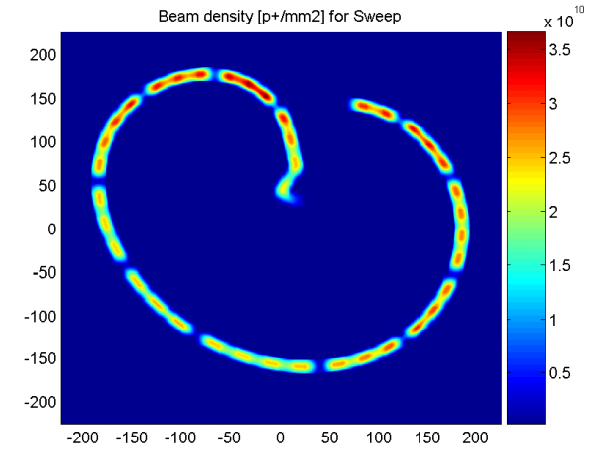
\includegraphics[width=0.5\textwidth]{figures/experiment/beamdump.png}
\caption{\url{https://www.semanticscholar.org/paper/A-Large-Diameter-Entrance-Window-for-the-LHC-Beam-Presland-Ramos/9344cf28c4853af4c4db01bce19d264d99ed2198}}
\label{fig:beamdump}
\end{figure}

When the beam has degraded to the point where it is no longer useful, it must be disposed of safely.
Over the course of several hours, the beam will loose intensity to the point where it is more efficient to dump the beam and replace it.
Occasionally an error in one of the LHC subsystems will be detected, and the beam is dumped as a precaution.
In both cases, the beam dump system is used to remove the beam from the machine while minimizing damage to its components.

There are three steps in disposing the beam. 
The first is to extract the beam from it's nominal orbit.
The second is to dilute the beam's density.
Finally the beam is absorbed in a material, where its energy is converted to radiation and heat. \cite{lhcDesignV1}

Focusing on one beam, it begins in its nominal orbit, when an abort is triggered. 
If the beam is in a safe state, the abort system will wait until the abort gap arrives to ramp up the extraction kicker magnets (MKD).
If the beam needs to be dumped immediately, the MKDs can ramp up outside the abort gap with minimal damage to the system.
The 15 copper wound magnets are powered by a bank of capacitors that can quickly energize the magnets in under 3.0~$\mu s$ to produce a field of 0.34~T. 
Once energized, the MKDs deflect the beam horizontally out of the ring.
The magnets remain on for 90~$\mu s$ to allow the full beam to exit the ring.

Next, the diluter kicker magnets (MKB) sweep out the beam in an ``e'' pattern as shown in Figure \ref{fig:beamdump}.
This spreads out the area where the beam will deposit its energy.
The diluter is built from four horizontal, and six vertical magnets that are powered by a sinusoidal current to produce the shape.
Like the MKDs, the MKBs are non-superconducting low-oxygen coper wound magnets.

The extraction septum magnets (MSD) have a septum (gap) for the extracted beam.
To allow the passage of the circulating beam, a low-field hole is drilled through the yoke.
The MSDs are responsible for deflecting the beam vertically.

Finally, beam comes to the Beam Dump Absorber Block (TDE).
This consists of carbon cylinders due to its high melting temperature and thermal shock resistance.
In particular, alternating layers of solid polycrystalline graphite cylinders and flexible graphite are used for a balance of solidity and flexibility.
The total length of carbon material is 7.7~m long.
To help reduce the thermal stress on the carbon, the TDE is cooled by water pipes.
Finally, the assembly is surrounded shielding made from old dipole yokes filled with concrete.

The MKD and MSD magnets used in the beam abort share a design with the magnets used to steer the beam into the rings during injection.
At the beam dump, the MKDs deflect horizontally while the MSDs deflect vertically.
At the injection points, it is reversed and the MKDs steer the beam horizontally while the MSDs steer it vertically.

\newpage

\subsection{History of the LHC}
\begin{itemize}
    \item LHC is an interesting story
    \item Run 1 lead to the physics discoveries that motivated VH
    \item Run 1 also lead to the development of the machine that enabled Run 2
\end{itemize}
\subsubsection{Run 1}
This is important because of the developments and understandings that lead to Run 2. But also for discovery of Higgs
\begin{itemize}
    \item Between 2010 and 2013, energies of 3.5-4 TeV \cite{lhcRun1}
    \item Bunch structure: bunches are 150ns (2010), 75ns (2011) and 50ns (2011/2012). \cite{lhcRun1}
    \item Beams consist of bunches, grouped together in trains. \cite{lhcRun1}
    \item \textbf{2010:} \cite{lhcRun1}
    \begin{itemize}
        \item Energy 3.5 TeV \cite{lhcRun1}
        \item Commissioning run at 1.2 TeV. Physics run at 3.5 TeV. \cite{lhcRun1}
        \item First injection February 27. First collisions march 30 2010, with two bunches. \cite{lhcRun1}
        \item Over the course of months, the number of bunches, and number of particles per bunch were increased. Reached 368 bunches October 10. \cite{lhcRun1}
        \item Beam losses, caused by UFO (unidentified falling objects).  Lead to about 60 beams being dumped. \cite{lhcRun1}
        \item Unexpected oscillations in beam tune continued from 2009 to 2010. Unclear of source. Called the hump. \cite{lhcRun1}
        \item Reached bunch spacing of 50 ns towards end \cite{lhcRun1}
    \end{itemize}
    \item \textbf{2011:} \cite{lhcRun1}
    \begin{itemize}
        \item Energy 3.5 TeV \cite{lhcRun1}
        \item First beams feb 19. 3 weeks recommissioning. \cite{lhcRun1}
        \item First physics beams march 13 with 32 bunches. Ramped up to 200 bunches, 75ns bunch spacing. \cite{lhcRun1}
        \item April 21 2011 luminosity of 4.6e33 $cm^{-2}s^{-1}$, which broke hadron lumi record from Tevatron. \cite{lhcRun1}
        \item Increased bunch intensities to 1.34$\times10^{11}$ ppb. \cite{lhcRun1}
        \item The hump disappears. \cite{lhcRun1}
        \item Mean stable beam time of 6.1 hrs. 33\% efficiency for stable beams. \cite{lhcRun1}
        \item 5.6 fb$^{-1}$ provided. \cite{lhcRun1}
    \end{itemize}
    \item \textbf{2012,2013:} \cite{lhcRun1}
    \begin{itemize}
        \item Energy increased to 4 TeV to increase Higgs production cross section. \cite{lhcRun1}
        \item First stable 4 TeV beams, 3 bunches, in April 5 2012 \cite{lhcRun1}
        \item First physics beam May 4. During this time, Higgs boson was discovered. \cite{lhcRun1}
        \item Nominal scheme was 1374 bunches, 50ns spacing. Due to gaps, this means 1368 colliding bunches in ATLAS. \cite{lhcRun1}
        \item There was a plan to have private bunches colliding only in LHCb. {\color{blue}Why?} \cite{lhcRun1}
        \item Bunch intensity peaked at 1.7e11 ppb. \cite{lhcRun1}
        \item 201 days with physics collisions, 36.5\% efficient stable beams. \cite{lhcRun1}
        \item 23.3 fb$^{-1}$ provided. \cite{lhcRun1}
        \item Typical emittance is 2-2.5 microns \cite{lhcRun1}
    \end{itemize}
    \item Cryo system in run 1 was most faulty, followed by injector systems. 25-30\% of fault time. \cite{lhcRun1}
    \item Best week in run 1 was june 2012, where 1.35 fb$^{-1}$ delivered. \cite{lhcRun1}
    \item Run 1 luminosity (page 7)\\ \cite{lhcRun1}
    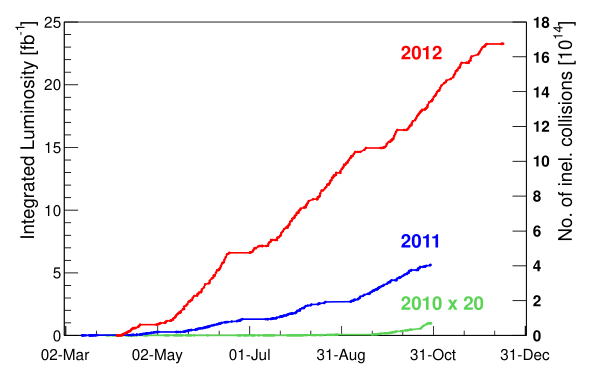
\includegraphics[width=0.8\textwidth]{figures/experiment/run1Lumi.png}
    \item \textbf{Beam Cycle} (probably, should use run2 resource) \cite{lhcRun1}
    \begin{itemize}
        \item Injection. Beam is ``scraped'' by transfer line collimator's. In run 1, about 2-4\% of the beam is lost. This done in SPS. The collimator jaws heat and outgas, so these are opened as soon as injection is finished. Rings are filled consecutively (as opposed to alternating bunches) because ALICE requested it (it reduces their background??). \cite{lhcRun1}
        \item Ramp. The ramping speed is limited by dipole current ramp rate of 10 A/s, which corresponds to 6 GeV/s. A ``flat top'' of 300 s, during which the tune decay is corrected for. \cite{lhcRun1}
        \item Separation/crossing angles. {\color{red} Warning, confused} Crossing angle is 170 micro radians. Separation is on the order of mm. Horizontal separation in P1,P2. Vertical in P5,P8. Hence in IR1 beam 1 moves downward/inside. \cite{lhcRun1}
        \item Collisions. When start, tails of bunches are expelled, leading to a brief drop in expected beam lifetime. The expected lifetime of the beam is optimized by reducing the chromaticity {\color{blue} \url{https://cds.cern.ch/record/302491/files/p77.pdf}(the change in linear parameters of transverse motion with beam energy).} HOW do they reduce chromaticity? \cite{lhcRun1}
        \item Tune. The beam is large during the ramp, and reduced during squeeze. \cite{lhcRun1}
        \item Collimators. Used for squeeze, used for betatron cleaning. Used to clean ``physics debris''. \cite{lhcRun1}
    \end{itemize}
\end{itemize}

\subsubsection{Run 2}
\begin{itemize}
    \item Between 2015 and 2018, beam energies of 6.5 TeV and provided lumi for 160 fb$^{-1}$. \cite{lhcRun2}
    \item Peak lumi is twice design, due to small emmitance and $\beta*$ of 30 cm. \cite{lhcRun2}
    \item Combined squeeze and ramp stages \cite{lhcRun2}
    \item 25 ns bunch spacing \cite{lhcRun2}
    \item \textbf{2015} \cite{lhcRun2}
    \begin{itemize}
        \item First year of 6.5 TeV energy, with 25 ns bunch spacing. \cite{lhcRun2}
        \item First beams April 5 2015. First stable beams June 3. \cite{lhcRun2}
        \item Relaxed $\beta*=80cm$, but due to shift in the ``optical waist'' position of the beam profile, the effective $\beta*=86cm$. (This leads to a slightly lower luminosity) \cite{lhcRun2}
        \item Reached 2244 bunches by end of year. Train length is 144 bunches. \cite{lhcRun2}
        \item Intensity ramp-up limited by heat load due to e-clouds. The heating effects the cryosystems. This despite efforts to scrub. Scrubbing done with low intensity bunches. \cite{lhcRun2}
        \item Beam 2 (15R8) had a UFO storm. The beamscrean was warmed to 80 K. An obstacle was left at bottom of the chamber called ULO (Unidentified lying object). The beam was steered around ULO.ULO remained an optical for full Run 2. ULO turned out to be plastic wrapping from installation. \cite{lhcRun2}
    \end{itemize}
    \item \textbf{2016} \cite{lhcRun2}
    \begin{itemize}
        \item First beams March 25. Target $\beta*=40cm$. 25ns bunch spacing. Again, limited to 144 bunches per train. Finally reached 2220 bunches. \cite{lhcRun2}
        \item June 26, LHC reached design lumi of 1.0e34 $cm^{-2}s^{-1}$. \cite{lhcRun2}
        \item Introduced BCMS (Batch Compression Merging and Splitting), lower transverse beam size with respect to the nominal production scheme. 20\% increase in Lumi1e 1.4e34 $cm^{-2}s^{-1}$.  \cite{lhcRun2}
        \item CMS received 5-10\% higher lumi, caused by oblong beams with low vertical emittance. The crossing plane for ATLAS is vertical, while for CMS it is horizontal. \cite{lhcRun2}
        \item In August 10, short circuit in one of dipole magnets in sector 12. Decision to replace the magnet, which lead to extended shutdown. \cite{lhcRun2}
    \end{itemize}
    \item \textbf{Batch Compression Merging and Splitting}
    \begin{itemize}\scriptsize
        \item The Linac 2 beam is continuous \cite{freyermuth}
        \item The PSB has 4 rings, each of which can be overfilled by injecting the Linac 2 beam in different positions. This overfilling increases emittance. \cite{freyermuth}
        \item The ``nominal'' scheme to fill the PS from the PSB was to inject 6 bunches. Each bunch is longitudinally split into 3 bunches, then by 2, and again by 2. Total 72 bunches. \cite{freyermuth}
        \item The BCMS scheme does two things. First, 8 (instead of 6) bunches are injected to PS and spread out over two PSB cycles. This reduces the emittance in the PSB, since the required intensity is lower, and injection is spread out over fewer turns. The 8 bunches are merged to 4, then split 3x2x2. Total 48 bunches, therefore more cycles needed to fill LHC, but get higher lumi. \cite{freyermuth}
    \end{itemize}
    \item \textbf{Luminosity Anti-leveling with crossing angle}
    \begin{itemize}\scriptsize
        \item At IP beams cross at an angle. This leads to 30-40\% loss in lumi. \cite{gorzawski}
        \item The angle is set based on the intensity of the beams. Prior to 2017, the beam angle was set based on the initial intensity of the beams. Peak beam intensity \cite{gorzawski}
        \item Some lumi can be recovered by reducing the crossing angle as the beams decay.  \cite{gorzawski}
        \item A study was conducted during machine development, using standard physics setup with few bunches. \cite{gorzawski}
        \item Leveling is slow, over the course of several minutes. The adjustments for the study were in steps of 20-85 microradians. \cite{gorzawski}
        \item Corresponding TCT (Collimators jaws) move. \cite{gorzawski}
        \item Study was successful, and recommended implementation is 2017  \cite{gorzawski}
    \end{itemize}
    \item \textbf{2017} \cite{lhcRun2}
    \begin{itemize}
        \item Introduced crossing angle anti-leveling. This procedure is applied in steps of 10 microradians. Gain of 3-4\% integrated lumi per fill. {\color{blue} More info from \cite{gorzawski}} \cite{lhcRun2}
        \item 16L2 problem. Seen during commissioning were sudden losses, and large background radiation. This due to condensed air that had leaked into the magnet replacement. Tried heating the beam screen, but failed and got worse. Big drop in lumi around August. Tried to reduce the e-cloud via 8b4e cleaning sequence. This reduced the cloud, and a high-lumi version was used for physics starting in august. \cite{lhcRun2}
        \item 8b4e is 8 beam bunches, four empty buckets. \cite{lhcRun2}
        \item Higher squeeze partway through run to beta*=30cm.  \cite{lhcRun2}
        \item Lumi record set at 2.06e34 $cm^{-2}s^{-1}$. This is too high for ATLAS, so was leveled to 1.5e34 $cm^{-2}s^{-1}$ for physics. \cite{lhcRun2}
        \item 50 fb$^{-1}$ delivered \cite{lhcRun2}
    \end{itemize}
    \item \textbf{2018} \cite{lhcRun2}
    \begin{itemize}
        \item Unable to remove all water trapped in beam pipe (16L2 problem). Heating the pipe exacerbated the situation.  \cite{lhcRun2}
        \item First beam April 30 {\color{red} probably March 30, this is a mistake?}, with target beta* at 30cm, with further squeeze to 25cm.  \cite{lhcRun2}
        \item First collisions on April 17, very quick. The intensity rampup was ahead of schedule. \cite{lhcRun2}
        \item The 16L2 problem resulted in beam dumps, and was rectified by running 900 bunch beams for several hours after a dump. \cite{lhcRun2}
        \item 66 fb$^{-1}$ delivered. \cite{lhcRun2}
    \end{itemize}
    \item Run 2 history: \cite{lhcRun2}
    \item Remember the marmot! \cite{lhcRun2}
    \begin{center}
    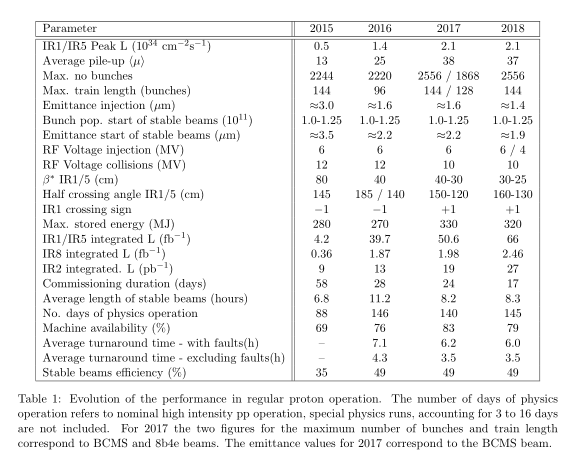
\includegraphics[width=1\textwidth]{figures/experiment/run2History.png}
    \end{center}
    \item Key points from table \cite{lhcRun2}
    \begin{itemize}
        \item Lumi, pileup, bunches \cite{lhcRun2}
        \item The leveling seen in Half crossing angle \cite{lhcRun2}
        \item Stored energy \cite{lhcRun2}
        \item Commissioning days \cite{lhcRun2}
        \item Physics days \cite{lhcRun2}
        \item Stable beam efficiency \cite{lhcRun2}
    \end{itemize}
    \item \textbf{Tunes} \cite{lhcRun2}
    \begin{itemize}
        \item The tune is adjusted over the course of injection, ramp, and collisions. \cite{lhcRun2}
    \end{itemize}
    \item \textbf{Chromaticity} \cite{lhcRun2}
    \begin{itemize}
        \item Controlled to $\pm$2 units during filling. Typical values Q are +20 during filling, +15 during operation. \cite{lhcRun2}
        \item See \cite{fuchsberger} for notes on chromaticity definition \cite{lhcRun2}
    \end{itemize}
    \item \textbf{Beam optics} \cite{lhcRun2}
    \begin{itemize}
        \item Local optics corrections were often reusable from year to year, which added reliability \cite{lhcRun2}
    \end{itemize}
    \item \textbf{Emittance} \cite{lhcRun2}
    \begin{itemize}
        \item Measured by BSRT, with 10\% accuracy. \cite{lhcRun2}
        \item Stable in 2016-18 at 1.4-1.7 micrometers, which increased to 1.9um after the ramp. \cite{lhcRun2}
        \item Horizontal emittance growth due to intra-beam scattering is estimated at 0.3-0.5um/hour. Measured at 0.3-0.5 + 0.6 um/hour, additional due to e-cloud \cite{lhcRun2}
        \item Vertical emittance growth is not expected, but appears possibly due to e-cloud, is 0.3-0.6um/hour. \cite{lhcRun2}
        \item Very small emittance growth due to synchrotron radiation. \cite{lhcRun2}
    \end{itemize}
    \item \textbf{RF and bunch length} \cite{lhcRun2}
    \begin{itemize}
        \item Target bunch length 1.1ns, which decreases due to synchrotron radiation over the course of the run. It is expanded periodically. \cite{lhcRun2}
        \item Nominal RF frequency is 400,789,711 \cite{lhcRun2}
    \end{itemize}
    \item \textbf{Electron clouds} \cite{lhcRun2}
    \begin{itemize}
        \item Work was done to mitigate, but impossible to remove them \cite{lhcRun2}
        \item Causes heat load in magnets. The heat load depends on the bunch pattern, indicating the source is from e-cloud. \cite{lhcRun2}
        \item High chromaticity helped stabilize beam in presence of e-clouds. \cite{lhcRun2}
    \end{itemize}
    \item \textbf{Machine Cycle} \cite{lhcRun2}
    \begin{enumerate}
        \item \textbf{Threading} The beam was injected with low bunch intensity, stopped on collimators at each IR. The trajectory is adjusted at each step. Then several orbits are averaged to get beam position, and steering takes place. With later runs, fewer corrections needed, since beam position does not change much more than 1-2mm. \cite{lhcRun2}
        \item \textbf{Injection} SPS bunchspacing is 250ns, and reduced to 200ns over Run 2 to get more bunches in. Steering was needed, at some times for fill. Steering done only for 12-bunch trains. Most fills only have one 12-bunch train to use for steering. \cite{lhcRun2}
        \item \textbf{Ramp and squeeze} Standard ramp time is 1210s. During ramp, squeeze is normally done after reaching 2 TeV. The ramping pattern is parabolic-exponential-linear-parabolic. Squeeze continues after ramp. Adjusting the beam optics is done in steps to avoid problem tunes. \cite{lhcRun2}
        \item \textbf{Collisions} Beams are steered to collide at all interaction points. \cite{lhcRun2}
        \item \textbf{Luminosity leveling} leveled to target 1.5e34$cm^{-2}s^{-1}$ when possible. Anti-leveling by adjusting crossing angle started in 2017 in steps of 10microradians. Leveling of beta* from 30cm to 27cm to 25cm added in 2018. \cite{lhcRun2}
        \item \textbf{Beam oscillations} Observed dipolar disturbances in beams during stable beams. Earthquakes were measured from as far away as New Zealand. Tidal deformation also observed. Distortions due to mechanical resonances as well. HL-LHC civil engineering also detected due to ground compactors. \\ \cite{lhcRun2}
        \begin{center}
        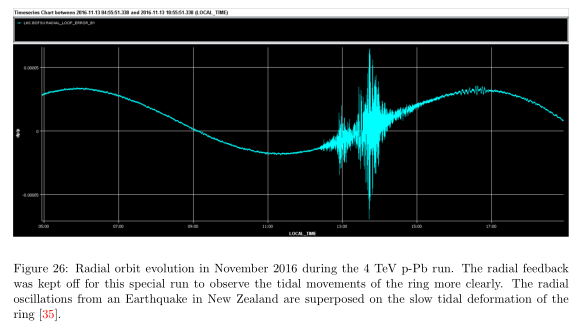
\includegraphics[width=0.6\textwidth]{figures/experiment/orbit.png}
        \end{center}
    \end{enumerate}
    \item UFO rates between 1-20 per hour, but only 4 dumps caused by UFO's in 2018. Sometimes due to quenches. \cite{lhcRun2}
    \item 16L2 problem. Probably caused by frozen water introduced after magnet replacement. Heating the beampipe lead to worse problem. Bunch structure changed to 8b4e bunch structure. Before 2018, 8L of nitrogen were flushed in. This improved the situation and BCMS beams could be used. Cleaning fills were used after dumps. \cite{lhcRun2}
    \item Heavy ion history \cite{lhcRun2}
    \begin{itemize}
        \item 2015 Pb-Pb \cite{lhcRun2}
        \item 2016 Pb-p \cite{lhcRun2}
        \item 2017 Xe \cite{lhcRun2}
        \item 2018 Pb-Pb \cite{lhcRun2}
    \end{itemize}
\end{itemize}

